\documentclass[pscyr,nonums]{hedlab}
\usepackage[russian]{babel}
\usepackage[utf8]{inputenc}
\usepackage{graphicx}
\usepackage{listings}

\labnum{2}
\labname{Введение в разработку WinPhone-приложений}
\student{Чечеткин И. А.}
\labdate{}

\lstset{inputencoding=utf8,
  language=[Sharp]C,
  basicstyle=\tiny,
  extendedchars=true,
  numbers=left,
  breaklines=true,
  literate=%
    {←}{{$\leftarrow$}}1
    {±}{{$\pm$}}1
    {√}{{$\sqrt{}$}}1
  }

\begin{document}
  \makeheader
  
  \emph{Цель работы:} 
  \begin{enumerate}
    \item познакомится с инструментами разработки WinPhone-приложения,
    \item разобрать структуру типичного WinPhone-приложения,
    \item научиться запускать приложение на эмуляторе.
  \end{enumerate}

  \vspace{2em}
  \emph{Калькулятор}
  
  \lstinputlisting[language=HTML,title={Страница приложения:}]{code/lab-2/MainPage.xaml}
  
  \lstinputlisting[title={Код приложения:}]{code/lab-2/MainPage.xaml.cs}  
  
  \begin{figure}[h!]
    \center
    Скриншот приложения: \\
    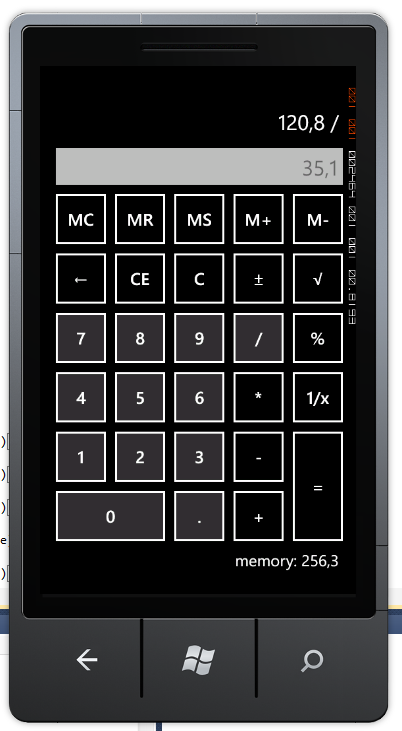
\includegraphics[width=.5\textwidth]{screen}
  \end{figure}
\end{document}
